\chapter{Stworzona architektura i zastosowane technologie}
\label{chapter:architektura}
W tym rozdziale opisana jest architektura zbudowanego systemu, wykorzystane
technologie i użyte narzędzia.
W rozdziale \ref{section:architekturasystemu} przedstawiono architekturę całego
systemu, w \ref{section:zastosowanetechnologie} omówione są technologie, a w
ostatniej części \ref{section:bibliotekiinarzedzia} wymienione są użyte biblioteki i
narzędzia.
\section{Architektura systemu}
\label{section:architekturasystemu}

\begin{figure}[ht!] \centering
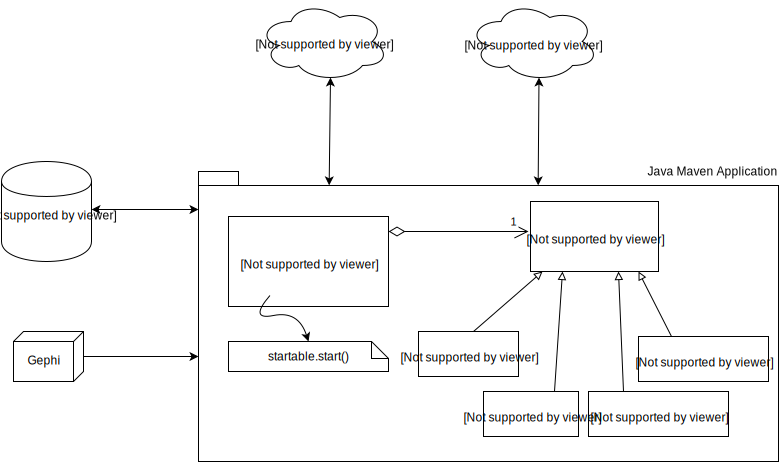
\includegraphics[width=140mm]{img/architektura.png}
\caption{Architektura systemu}
\label{image:architektura-systemu}
\end{figure}
System została zbudowany jako pojedyncza aplikacji Javowa, w której zostały
zaimplementowane wszystkie potrzebne mechanizmy.
Aplikacja ta komunikuje się z pojedynczą bazą danych, w której zawarte są
wszystkie rekordy potrzebne zarówno do zbierania danych jak i te, które są
wynikiem analiz. Dodatkowo odpowiada ona za komunikację z usługami w chmurze --
czyli zbieraniem danych z Twittera i \textit{georeversingiem} lokalizacji
\rref{subsection:modelgeolokacji} z Open Street Map. Wszystkie analizy zebranych
danych również zostały przeprowadzone przy użyciu aplikacji Javowej.

Oprócz niej wykorzystano także program Gephi, którego wyniki działania zapisano
do plików, a następnie przy użyciu wyżej wymienionej aplikacji przeparsowano i
umieszczono w bazie danych.

Wewnątrz aplikacji zaimplementowano między innymi moduł do zbierania danych z
Twittera (na podstawie podanych słów kluczowych), moduł związany z
przeprowadzeniem całego procesu analizy sentymentu -- od budowy słownika do
zanalizowania pojedynczych wpisów, moduł związany z analizą zebranych danych,
a także kod odpowiedzialny za operacje związane z geolokacją.

\section{Zastosowane technologie}
\label{section:zastosowanetechnologie}
% java, postgres, sql, git
Główną technologią użytą podczas prac był język Java. Oprócz niego wymienić
należy także:
\begin{itemize}
  \item baza danych -- PostgreSQL\footnote{www.postgresql.org},
  \item budowanie aplikacji -- Apache Maven\footnote{www.maven.apache.org},
  \item system kontroli wersji -- Git\footnote{www.git-scm.com} z 
  repozytorium na GitHub\footnote{www.github.com},
  \item wizualizacja wpisów na mapie -- CartoDB\footnote{www.cartodb},
  narzędzie webowe pozwalające na wyświetlanie danych posiadających współrzędne
  geograficzne na mapie świata.
\end{itemize}
\section{Wykorzystane biblioteki i narzędzia}
\label{section:bibliotekiinarzedzia}
% Twitter API, CartoDB, OSMap, GMap, GCharts, CartoDB, Gephi
Najważniejsze wykorzystane biblioteki:
\begin{itemize}
  \item Twitter4J\footnote{www.twitter4j.org} -- biblioteka Javowa ułatwiająca 
  korzystanie z Twitter API, użyta do zbierania \mbox{danych z Twittera,}
  
  \item Hibernate\footnote{www.hibernate.org} -- framework 
  ORM (Object Relational Mapping --  mapowanie obiektowo-relacyjne) do 
  komunikacji z bazą danych,
  
  \item PostGIS\footnote{www.postgis.net} -- rozszerzenie do bazy PostgreSQL
  dodające funkcje geograficzne, przy pomocy którego możliwe jest między
  innymi określenie odległości między dwoma punktami (znając ich współrzędne)
  
  
  
  \item Google Guice\footnote{www.github.com/google/guice}, 
  JBoss Weld\footnote{www.weld.cdi-spec.org} -- biblioteki pozwalające zastosować
  wstrzykiwanie zależności w desktopowej aplikacji Javowej,
  
  \item Google Guava\footnote{www.code.google.com/p/guava-libraries}, 
  Apache Commons\footnote{www.commons.apache.org}, 
  Apache Log4J\footnote{www.logging.apache.org/log4j}, 
  Joda Time\footnote{www.joda.org/joda-time} -- biblioteki
  usprawniające programowanie w Javie,
  
  \item JUnit\footnote{www.junit.org} -- framework do pisania i uruchamiana
  testów automatycznych.
\end{itemize}


\section{Baza danych}
Jak zostało już wspomniane użyty został system zarządzania bazą danych
PostgreSQL.
Na rysunku \ref{image:schemat-bazy} zaprezentowany jest schemat bazy danych. W
przedstawionych tabelach zostały zapisane wszystkie informacje potrzebne do
pobierania danych z nasłuchiwanych meczów.

Opis najważniejszych tabel został załączony na końcu pracy.

\begin{figure}[ht!]
\centering
\includegraphics[width=160mm]{img/db-schema-intellij.png}
\caption{Schemat bazy danych}
\label{image:schemat-bazy}
\end{figure}